\chapter{Mécanique des milieux continus} \label{chap:Ch01}
Les éléments de base de la MMC (cinématique des milieux continus, variables lagrangiennes et eulériennes, dérivées particulaires, -- description des efforts intérieurs, contraintes) ont présentés dans le cours d'introduction à la MMC.
Nous nous bornerons donc, dans ce chapitre, à les replacer dans un contexte «~Mécanique des Solides~». 
En particulier, nous ne donnerons pas le détail des démonstrations. 
Le lecteur pourra se référer aux traités classiques (voir \cite{Germain-62,Germain-73,Mandel-66,Mandel-74,Gontier-69,Roy-66,Sedov-71,Eringen-67,Prager-61,Lai-78}).
\section{Lois de conservation} \label{sec:Ch01-1}
\subsection{Lois de la physique} \label{ssec:Ch01-1.1}
En MMC, on appelle «~loi de conservation~» la traduction mathématique des lois de la physique.
Dans le cadre d'une schématisation donnée, elles sont donc universelles. 
Par exemple, dans le cas de la MMC classique (qui fait l'objet de ce cours), il faut écrire pour tout domaine matériel $D$:
\begin{itemize}
    \item la loi de conservation de la masse;
    \item la loi fondamentale de la dynamique qui se décompose en deux parties: conservation de la quantité de mouvement et conservation du moment cinétique.
\end{itemize}
En introduisant la masse spécifique, c'est-à-dire la masse par unité de volume, $\rho$, la loi de conservation de la masse s'écrit:
\begin{equation}
    \frac{\ud}{\ud t}\iiint_D \rho \ud v =0
    \label{eq:Ch01-001}
\end{equation}
où $\frac{\ud}{\ud t}$ est la dérivée «~particulaire~», c'est à dire la dérivée obtenue en suivant le domaine $D$ dans son mouvement (voir par exemple~\cite{Germain-73}).

Pour écrire la loi fondamentale, il faut schématiser les efforts exercés sur $D$:
\begin{itemize}
    \item les efforts à distance -- la pesanteur par exemple -- sont caractérisés par une densité volumique $\vec{f}$ ($\vec{f}=\rho \vec{g}$ par exemple pour la pesanteur);
    \item les efforts de contact, c'est-à-dire les efforts exercés sur $D$ à travers la frontière $\partial D$ de $D$ seront caractérisés par une densité superficielle de force $\vec{T}$ en vertu du:
\end{itemize}
\begin{center}
    \psset{xunit=1.2cm,yunit=1.2cm}
    \begin{pspicture}(0,-0.5)(6,2)
        %\psgrid
        \psccurve(0.5,1)(2,1.8)(4,1.2)(4,0.4)
        \rput(2.5,1){$D$}
        \rput(0.5,1.7){$\partial D$}
        \psline{->}(4,0.4)(5.5,0.2)
        \psline{->}(4,0.4)(4.5,0)
        \rput(4.3,-0.15){$\vec{n}$}
        \rput(5.6,0.4){$\vec{T}$}
        \rput(3.8,0.5){$M$}
    \end{pspicture}
\end{center}
\begin{Postulat}[Postulat de Cauchy.]
    \hfill
    \begin{enumerate}[(a)]
        \item Les efforts de contact exercés sur $D$ à travers $\partial D$ sont schématisés par une densité superficielle de force $\vec{T}$;
        \item Cette densité superficielle $\vec{T}$ ne dépend que du point $M$ considéré et du vecteur normal $\vec{n}$ à $\partial D$: $\vec{T}(M,\vec{n})$.
    \end{enumerate}
\end{Postulat}

Malgré son apparence toute naturelle, ce postulat n'est pas le seul possible.
On peut par exemple considérer que ces efforts de contact sont schématisés par une densité superficielle de force $\vec{T}$ et de moment $\vec{M}$ -- on parle alors de «~milieux avec couples de contraintes~», exemple embryonnaire de milieux avec microstructure (nous reparlerons de ces milieux au paragraphe~\ref{ssec:Ch01-2.2}).

Moyennant ces schématisations, la loi fondamentale de la dynamique: «~La dérivée par rapport au temps du torseur des quantités de mouvement d'un domaine matériel $D$ quelconque est égale au torseur de tous les efforts extérieurs (à distance et de contact) appliqués à $D$~» va se traduire par les deux lois de conservation:
\begin{itemize}
    \item de la quantité de mouvement
        \begin{equation}
            \frac{\ud}{\ud t}\iiint_D \rho\vec{V} \ud v =\iint_{\partial D}\vec{T}\ud s+\iiint_D\vec{f}\ud v
            \label{eq:Ch01-002}
        \end{equation}
    \item du moment cinétique (par rapport à 0 fixe)
        \begin{equation}
            \frac{\ud}{\ud t}\iiint_D \rho\vec{OM}\wedge\vec{V} \ud v =\iint_{\partial D}\vec{OM}\wedge\vec{T}\ud s+\iiint_D\vec{OM}\wedge\vec{f}\ud v
            \label{eq:Ch01-003}
        \end{equation}
\end{itemize}
De manière générale, une loi de conservation exprime un bilan:
\begin{equation}
    \frac{\ud}{\ud t}\iiint_D \mathcal{A} \ud v =\iint_{\partial D}\alpha\ud S +\iiint_D A\ud v
    \label{eq:Ch01-004}
\end{equation}
valable pour tout domaine matériel $D$: la variation d'une quantité (de densité volumique $\mathcal{A}$) provient d'une part de la production interne de cette quantité (densité volumique $\mathcal{A}$) et d'autre part des échanges avec l'extérieur à travers $\partial D$ (densité surfacique $\alpha$).

Les trois lois de conservation qU1 nous intéressent \eqref{eq:Ch01-001}, \eqref{eq:Ch01-002} et \eqref{eq:Ch01-003} rentrent dans ce cadre d'après le tableau suivant:
\begin{table}[h]\centering
    \begin{tabular}{l|c|c|c|}
        & A & $\alpha$ & A \\\hline
        masse & $\rho$ & 0 & 0\\\hline
        quantité de mouvement & $\rho V_i$ & $T_i$ & $f_i$ \\\hline
        moment cinétique & $\rho \varepsilon_{ijk}x_j V_k$ & $\varepsilon_{ijk}x_j V_k$ & $\varepsilon_{ijk}x_j k_k$
    \end{tabular}
    %\caption{Quantités mécaniques}
\end{table}
où l'on a introduit les composantes des vecteurs qui interviennent dans \eqref{eq:Ch01-002} et \eqref{eq:Ch01-003} (voir annexe~\ref{Ann:A} pour l'expression des produits vectoriels qui interviennent dans \eqref{eq:Ch01-003}).
Nous verrons que paragraphe~\ref{ssec:Ch01-3.1} que la loi de conservation de l'énergie rentre également dans ce cadre.
\subsection{Étude d'une loi de conservation} \label{ssec:Ch01-1.2}
Pour utiliser la loi de conservation générale~\eqref{eq:Ch01-004}, il faut expliciter la dérivée particulaire d'une intégrale de volume.
\begin{lem}[Dérivée particulaire d'une intégrale de volume]\label{lem:Ch01-1}
    \begin{equation}
        \frac{\ud}{\ud t}\iiint_D \mathcal{A} \ud v =\iiint_D\frac{\partial \mathcal{A}}{\partial t}\ud S+\iint_{\partial D}\mathcal{A}\vec{V}\cdot\vec{n}\ud S
        \label{eq:Ch01-005}
    \end{equation}
\end{lem}
\begin{multicols}{2}
    \raggedcolumns
    \setcounter{unbalance}{2}
Ce résultat classique peut s'obtenir de diverses manières.
L'idée essentielle est que la variation de l'énergie provient de:
\begin{enumerate}
    \item la variation de la quantité $\mathcal{A}$;
    \item la variation du domaine d'intégration.
\end{enumerate}
\columnbreak
\begin{center}
    \psfrag{D1}{$D_I$}
    \psfrag{D2}{$D_{II}$}
    \psfrag{D3}{$D_{III}$}
    \psfrag{Vdt}{$\vec{V} \mathrm{d}t$}
    \psfrag{Dtdt}{$D\left( t+\mathrm{d}t \right)$}
    \psfrag{Dt}{$D\left( t \right)$}
    \psfrag{t}{\footnotesize $\theta$}
    \psfrag{n}{$\vec{n}$}
    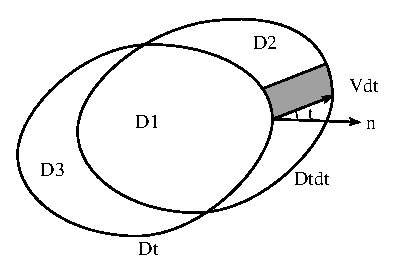
\includegraphics[scale=1]{../images/T1_Ch01-0002.eps}
\end{center}
\end{multicols}

Posant $J(t)=\iiint_{D(t)} \mathcal{A}(x,t) \ud v$, on peut écrire:
\begin{equation*}
    \begin{aligned}
        J(t+\ud t)-J(t) & =\iiint_{D(t+\ud t)} \mathcal{A}(x,t+\ud t) \ud v-\iiint_{D(t)} \mathcal{A}(x,t) \ud v\\
                        & =\iiint_{D_I} \left[\mathcal{A}(x,t+\ud t)-\mathcal{A}(x,t)\right] \ud v+\iiint_{D_{II}} \mathcal{A}(x,t+\ud t) \ud v-\iiint_{D_{III}} \mathcal{A}(x,t) \ud v\\
                        & =\left[\iiint_{D} \frac{\partial \mathcal{A}}{\partial t}(x,t) \ud v\right]\ud t+ \left[\iint_{\partial D} \mathcal{A}\vec{V}\cdot\vec{n} \ud s\right]\ud t
    \end{aligned}
\end{equation*}
en remarquant que pour $II$ ou $III$, l'élément de volume $\ud v$ (hachuré sur la figure ci-contre) est donné par:
\begin{equation*}
    \ud v=\pm V \ud t \cdot \ud S \cdot \cos\theta = \pm \vec{V}\cdot\vec{n} \ud S \ud t
\end{equation*}
On trouvera des démonstrations plus détaillées et plus rigoureuses dans \cite{Germain-62,Germain-73,Mandel-66,Gontier-69} entre autres.

En utilisant le théorème de la divergence (Annexe~\ref{Ann:A}) et la formule donnant la dérivée particulaire $\mathcal{A}$:
\begin{equation*}
    \frac{\ud \mathcal{A}}{\ud t}=\frac{\partial \mathcal{A}}{\partial t}+\mathcal{A}_{,i}V_i
\end{equation*}
(où on a utilisé la convention de sommation et la notation $f_{,i}=\partial f/\partial x_i$ -- voir Annexe~\ref{Ann:A}), on peut transformer~\eqref{eq:Ch01-005} en:
\begin{equation}
    \frac{\ud}{\ud t}\iiint_{D} \mathcal{A} \ud v=\iiint_{D}\left\{\frac{\partial\mathcal{A}}{\partial t}+(\mathcal{A}V_i)_{,i}\right\} \ud v=\iiint_{D} \left\{\frac{\ud\mathcal{A}}{\ud t}+\mathcal{A}\dive\vec{V}\right\} \ud v
    \label{eq:Ch01-006}
\end{equation}
Par une hypothèse analogue au Postulat de Cauchy, on suppose que la densité surfacique $\alpha$ dépend uniquement du point considéré et de la normale $\vec{n}$: $\alpha(M,\vec{n})$.
Moyennant des hypothèses de continuité que nous ne préciserons pas davantage, on montre alors:

\begin{lem}
    \hfill
    \begin{enumerate}[(a)]
        \item $\alpha(M,-\vec{n}) =-\alpha(M,\vec{n})$
        \item En un point donné $M$, il existe un flux $\vec{a}(M)$ tel que:
        \begin{equation}
            \alpha(M,\vec{n}) =a_i(M)n_i=\vec{a}\cdot\vec{n}
            \label{eq:Ch01-007}
        \end{equation}
    \end{enumerate}
    \label{lem:Ch01-2}
\end{lem}

\begin{wrapfigure}[3]{l}{.2\textwidth}
    \vskip-1.5em
    \centering
    \psfrag{dS}{\scriptsize $\ud S$}
    \psfrag{n}{\scriptsize $\vec n$}
    \psfrag{-n}{\scriptsize $-\vec n$}
    \psfrag{e}{\scriptsize $\varepsilon$}
    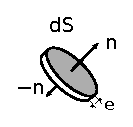
\includegraphics[clip]{../images/T1_Ch01-0003.eps}%\vspace{.2cm}
\end{wrapfigure}
\noindent Le point a) exprime simplement que ce qui rentre dans $D$ est l'opposé de ce qui en sort.
Lorsque $\varepsilon\rightarrow 0$, les seuls termes qui subsistent sont ceux relatifs aux deux faces, et \eqref{eq:Ch01-004} donne le point a).
\vspace{1em}

\begin{wrapfigure}[5]{r}{.2\textwidth}
    \vskip-2em
    \centering
    \psfrag{x1}{\scriptsize $x_1$}
    \psfrag{x2}{\scriptsize $x_2$}
    \psfrag{x3}{\scriptsize $x_3$}
    \psfrag{M0}{\scriptsize $M_0$}
    \psfrag{M1}{\scriptsize $M_1$}
    \psfrag{M2}{\scriptsize $M_2$}
    \psfrag{M3}{\scriptsize $M_3$}
    \psfrag{-e1}{\scriptsize $-\vec e_1$}
    \psfrag{-e2}{\scriptsize $-\vec e_2$}
    \psfrag{-e3}{\scriptsize $-\vec e_3$}
    \psfrag{n}{\scriptsize $\vec n$}
    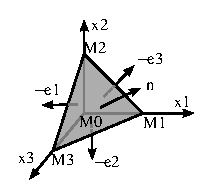
\includegraphics[clip]{../images/T1_Ch01-0004.eps}
\end{wrapfigure}
\noindent Pour démontrer le point b), on écrit~\eqref{eq:Ch01-004} pour un domaine $D$ en forme de tétraèdre $M_OM_1M_2M_3$, la face $M_1M_2M_3$ restant perpendiculaire au vecteur $\vec{n}$ donné.
Lorsque les dimensions du tétraèdre tendent vers zéro, la fonction $\alpha(M,\vec{n})$ reste à peu près constante en et ne dépend donc que de $\vec{n}$.

De plus, seule subsiste dans \eqref{eq:Ch01-004} l'intégrale de surface:
\begin{equation*}
    0=\iint_{M_1M_2M_3}\alpha(\vec{n}) \ud S+\iint_{M_0M_1M_2}\alpha(-\vec{e}_3) \ud S+ \iint_{M_0M_1M_3}\alpha(-\vec{e}_2) \ud S+\iint_{M_0M_2M_3}\alpha(-\vec{e}_1) \ud S
\end{equation*}
Si on note $S$ la surface de la face $M_1M_2M_3$ et $S_1$, $S_2$, $S_3$ celles de $M_OM_2M_3$, $M_OM_1M_3$, $M_0M_1M_2$ respectivement, il vient:
\begin{equation*}
    0 = \alpha(\vec{n})S+\alpha(-\vec{e}_3)S_3+\alpha(-\vec{e}_2)S_2+\alpha(-\vec{e}_1)S_1
\end{equation*}
soit, en utilisant a), en posant $a_i=\alpha(\vec{e}_i)$ et en remarquant que $S_i=\cos(\vec{e}_i,\vec{n})S=n_iS$:
\begin{equation*}
    \alpha(\vec{n})=a_in_i
\end{equation*}
Par utilisation de ces deux lemmes, on obtient la forme locale ou différentielle de la loi de conservation~\eqref{eq:Ch01-004}:
\begin{thm}
    \begin{equation}
        \frac{\ud \mathcal{A}}{\ud t} = -\mathcal{A}V_{i,i} + a_{i,i} + A
        \label{eq:Ch01-008}
    \end{equation}
    \label{thm:Ch01-1}
\end{thm}
\begin{proof}[Première démonstration]
    On utilise le théorème de la divergence pour transformer dans \eqref{eq:Ch01-004} l'intégrale de surface.
    Il vient:
    \begin{equation*}
        \iiint_D\left(\frac{\ud \mathcal{A}}{\ud t}+\mathcal{A}_{i,i}-a_{i,i}-A\right)\ud v=0
    \end{equation*}
    Cette égalité devant avoir lieu pour tout domaine $D$, on en tire la nullité de la quantité intégrée.
\end{proof}

\begin{proof}[Deuxième démonstration]
    On écrit la loi de conservation \eqref{eq:Ch01-004} en choisissant comme domaine $D$ un petit parallélépipède de côtés $h_1$, $h_2$, $h_3$.
    En utilisant le \tmp{lemme X}, on obtient en première approximation:
    \begin{align*}
        \frac{\ud}{\ud t}\iiint_D \mathcal{A} \ud v &= \iiint_D\left(\frac{\ud \mathcal{A}}{\ud t}+\mathcal{A}\dive \vec{V}\right)\ud v \\
        & \simeq \left(\frac{\ud \mathcal{A}}{\ud t}+\mathcal{A}\dive \vec{V}\right) h_1h_2h_3
    \end{align*}
    avec l'hypothèse $\iiint_D A \ud v =A h_1h_2h_3$.

    Pour l'intégrale de surface, on obtient:
    \begin{align*}
        \iint_{\partial D}\alpha \ud S & =\iint_{\partial D}\left(a_1n_1+a_2n_2+a_3n_3\right)\ud S \\
                                       & =\iint_{S_1}\quad \cdots \text{ permutation circulaire}\\
                                       & =\iint_{S_1} \left[a_1(x_1+h_1)-a_1(x_1)\right] \ud x_1 \ud x_2 + \cdots
    \end{align*}
    puisque $\vec{n}= (1,0,0)$ sur $S_1(x_1+h_1)$ et $\vec{n} = (-1,0,0)$ sur $S_1(x_1)$.
    Finalement il vient:
    \begin{equation*}
        \iint_{\partial D}\alpha \ud S=\left(\frac{\partial a_1}{\partial x_1}h_1\right)h_2h_3+\cdots=\frac{\partial a_i}{\partial x_i}h_1 h_2 h_3
    \end{equation*}
    d'où le résultat.
\end{proof}
\rput(11.8,8.5){%
\psfrag{x1}{\scriptsize $x_1$}
\psfrag{x2}{\scriptsize $x_2$}
\psfrag{x3}{\scriptsize $x_3$}
\psfrag{h1}{\scriptsize $h_1$}
\psfrag{h2}{\scriptsize $h_2$}
\psfrag{h3}{\scriptsize $h_3$}
\psfrag{e1}{\scriptsize $\vec e_1$}
\psfrag{e2}{\scriptsize $\vec e_2$}
\psfrag{e3}{\scriptsize $\vec e_3$}
\psfrag{-e1}{\scriptsize $-\vec e_1$}
\psfrag{-e2}{\scriptsize $-\vec e_2$}
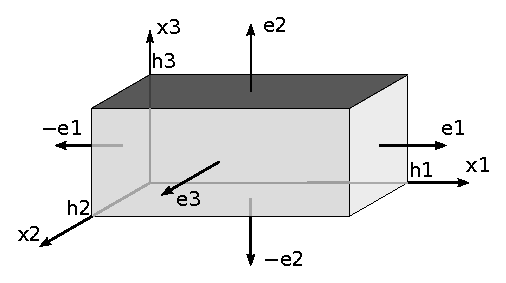
\includegraphics[width=7cm]{../images/T1_Ch01-0005.eps}}
Cette forme locale suppose la continuité des différentes quantités en cause.
En présence d'une surface de discontinuité $\Sigma$ se déplaçant à la vitesse $\vec{V}$, on définit la vitesse relative du choc $U$ par:
\begin{equation}
    U=(\vec{W}-\vec{V})\cdot \vec{N}
    \label{eq:Ch01-009}
\end{equation}
\begin{wrapfigure}[7]{l}{.3\textwidth}
    \psfrag{D}{\scriptsize $D$}
    \psfrag{S}{\scriptsize $\Sigma$}
    \psfrag{W}{\scriptsize $\vec W$}
    \psfrag{N}{\scriptsize $\vec N$}
    \includegraphics{../images/T1_Ch01-0006}
\end{wrapfigure}
On peut alors montrer (voir \cite{Germain-73}) que l'équation locale~\eqref{eq:Ch01-008} doit être complétée par une «~équation aux discontinuités~»:
\begin{equation}
    \llbracket\mathcal{A}U + a_iN_i\rrbracket = 0 
    \label{eq:Ch01-010}
\end{equation}
en désignant par $\llbracket h \rrbracket h(M^+)-h(M^-)$ le saut d'une grandeur à travers $\Sigma$.

L'application du Théorème~\ref{thm:Ch01-1} à la loi de conservation de la masse~\eqref{eq:Ch01-001} donne:
\begin{equation}
    \frac{\ud \rho}{\ud t}+\rho \dive \vec{V}=0
    \label{eq:Ch01-011}
\end{equation}
c'est l'équation de continuité.
Un calcul simple montre alors que:
\begin{equation*}
    \frac{\ud\mathcal{A}}{\ud t}+\mathcal{A}\dive \vec{V}=\rho\left\{\frac{1}{\rho}\frac{\ud \mathcal{A}}{\ud t}-\frac{1}{\rho^2}\mathcal{A}\frac{\ud \rho}{\ud t}\right\}=\rho \frac{\ud}{\ud t}\left(\frac{\mathcal{A}}{\rho}\right)
\end{equation*}
Le Lemme~\ref{lem:Ch01-1} et le Théorème~\ref{thm:Ch01-1} deviennent alors:
\begin{lem}[Lemme~\ref{lem:Ch01-1}']
    \begin{equation}
        \frac{\ud}{\ud t}\iiint_D\mathcal{A}\ud v=\iiint_D\rho\frac{\ud}{\ud t}\left(\frac{\mathcal{A}}{\rho}\right)(12)
        \label{eq:Ch01-012}
    \end{equation}
    \label{lem:Ch01-1p}
\end{lem}

\begin{thm}[Théorème~\ref{thm:Ch01-1}']
    \begin{equation}
        \rho\frac{\ud}{\ud t}\left(\frac{\mathcal{A}}{\rho}\right)=A+a_{i,i}(13)
        \label{eq:Ch01-013}
    \end{equation}
    \label{thm:Ch01-1p}
\end{thm}
Ces deux formes sont très utiles, car les quantités physiques sont plus souvent définies par leur densité massique $\mathcal{A}/\rho$ que volumique $\mathcal{A}$.
\subsection{Utilisation de la loi fondamentale} \label{ssec:Ch01-1.3}
L'application du Lemme~\ref{lem:Ch01-2} à la loi de conservation de la quantité de mouvement~\eqref{eq:Ch01-002} (en prenant $\alpha=T_i$ permet d'introduire le \emph{tenseur des contraintes} $\sigma_{ij}$
système de 9 quantités, tel que:
\begin{equation}
    T_i=\sigma_{ij}n_j
    \label{eq:Ch01-014}
\end{equation}
Le chapitre~\ref{chap:Ch02} sera consacré à l'étude de ce «~tenseur des contraintes~».

L'application du Théorème~\ref{thm:Ch01-1p} à la loi de conservation de la quantité de mouvement \eqref{eq:Ch01-002} donne alors \emph{l'équation du mouvement}:
\begin{equation}
    \rho\gamma_i=\rho\frac{\ud V_i}{\ud t}=\sigma_{ij,j}+f_i
    \label{eq:Ch01-015}
\end{equation}
où $\gamma_i$ désigne l'accélération:
\begin{equation}
    \gamma_i=\frac{\ud V_i}{\ud t}=\frac{\partial V_i}{\partial t}+V_{i,j}V_j
    \label{eq:Ch01-016}
\end{equation}
Dans la suite de ce cours, on s'intéressera essentiellement aux problèmes statiques.
L'équation du mouvement~\eqref{eq:Ch01-015} devient alors \emph{l'équation d'équilibre}:
\begin{equation}
    \sigma_{ij,j}+f_i=0
    \label{eq:Ch01-017}
\end{equation}
système de 3 équations scalaires ($i=1,2,3$):
\begin{equation}
    \begin{aligned}
        &\frac{\partial \sigma_{11}}{\partial x_1}+\frac{\partial \sigma_{12}}{\partial x_2}+\frac{\partial \sigma_{13}}{\partial x_3}+f_1=0\\
        &\frac{\partial \sigma_{21}}{\partial x_1}+\frac{\partial \sigma_{22}}{\partial x_2}+\frac{\partial \sigma_{23}}{\partial x_3}+f_2=0\\
        &\frac{\partial \sigma_{31}}{\partial x_1}+\frac{\partial \sigma_{32}}{\partial x_2}+\frac{\partial \sigma_{33}}{\partial x_3}+f_3=0
    \end{aligned}
    \label{eq:Ch01-018}
\end{equation}
qui traduisent localement l'équilibre du milieu continu.

La loi de conservation du moment cinétique s'étudie de la même manière: on applique le Théorème~\ref{thm:Ch01-1p} avec $\mathcal{A}/\rho=\varepsilon_{ijk}a_jV_k$, $\alpha=\varepsilon_{ijk}x_jT_k=\varepsilon_{ijk}x_j\sigma_{kl}n_l$ d'après \eqref{eq:Ch01-014}, et $A=\varepsilon_{ijk}x_jk_k$.
Il vient:
\begin{equation*}
    \rho \frac{\ud}{\ud t}(\varepsilon_{ijk}x_jV_k)=(\varepsilon_{ijk}x_j\sigma_{kl})_{,l}+\varepsilon_{ijk}x_jf_k
\end{equation*}
On développe cette relation en remarquant que:
\begin{equation*}
    \frac{\ud x_j}{\ud t}=V_j, \qquad x_{j,l}=\frac{\partial x_j}{\partial x_l}=\delta_{jl}
\end{equation*}
où $\delta_{jl}$ est le symbole de Kronecker:
\begin{equation*}
    \rho \varepsilon_{ijk}V_jV_k+\rho\varepsilon_{ijk}x_j\gamma_k=\varepsilon_{ijk}\delta_{jl}\sigma_{kl}+\varepsilon_{ijk}x_j\sigma_{kl,l}+ \varepsilon_{ijk}x_jf_k
\end{equation*}
Le premier terme disparaît car $\varepsilon_{ijk}$ est antisymétrique en $j$ et $k$.
Il reste:
\begin{equation*} 
    \varepsilon_{ijk}x_j(\rho\gamma_k-\sigma_{kl,l}-f_k)-\varepsilon_{ijk}\sigma_{jk}=0
\end{equation*}
Le premier terme s'annule d'après \eqref{eq:Ch01-015} et on obtient finalement $\varepsilon_{ijk}\sigma_{jk}=0$ c'est à dire:
\begin{equation}
    \sigma_{ij}=\sigma_{ji}
    \label{eq:Ch01-019}
\end{equation}
Le tenseur des contraintes est symétrique.
\begin{displaymath}
    \sigma_{12} = \sigma_{21}, \quad \sigma_{13}= \sigma_{31}, \quad \sigma_{23} = \sigma_{32}
\end{displaymath}
Ainsi la loi fondamentale de la dynamique est, sous forme locale, équivalente â l'équation du mouvement~\eqref{eq:Ch01-015} avec un tenseur des contraintes symétrique.
A nouveau ces résultats supposent la continuité des fonctions en cause.
En présence d'une surface de discontinuité $\Sigma$, il faut rajouter les relations de discontinuité \eqref{eq:Ch01-010} qui donnent:
\begin{itemize}
     \item pour la conservation de la masse:
        \begin{equation}
            \llbracket \rho U \rrbracket=0, \qquad \rho^+(\vec{W}-\vec{V}^+)\cdot \vec{N} =\rho^-(\vec{W}-\vec{V}^-)\cdot \vec{N}
            \label{eq:Ch01-020}
        \end{equation}
    \item pour la conservation de la quantité de mouvement:
    \begin{equation}
        \llbracket \rho U V_i +\sigma_{ij}N_j \rrbracket=0
        \label{eq:Ch01-021}
    \end{equation}
\end{itemize}
tandis que l'équation correspondante pour la conservation du moment cinétique est automatiquement vérifiée si \eqref{eq:Ch01-022} l'est.

Dans le cas statique, ces relations de discontinuité se ramènent à la seule condition:
\begin{equation}
    \llbracket\sigma_{ij}N_j\rrbracket=0,\qquad \vec{T}^+(\vec{N})=\vec{T}^-(\vec{N})
    \label{eq:Ch01-022}
\end{equation}
exprimant la continuité du vecteur $\vec{T}$.
Nous y reviendrons au chapitre~\ref{chap:Ch02}.
\section{Puissances virtuelles} \label{sec:Ch01-2}
\subsection{Théorème des puissances virtuelles} \label{ssec:Ch01-2.1}
Pour un système quelconque un mouvement virtuel est un mouvement possible de ce système mouvement «~virtuel~» par opposition au mouvement «~réel~» qui est celui qui se réalise effectivement par suite des efforts appliqués.
De même une «~vitesse virtuelle~» est une répartition de vitesse possible.
Pour un milieu continu déformable, une vitesse virtuelle sera définie par un champ de vitesses virtuelles $\displaystyle{\mathop{V}^{*}}_i(x)$, c'est à dire par un champ de vecteurs $\displaystyle{\mathop{V}^{*}}_i$ défini sur le solide $\Omega$.

Nous partons donc de l'équation du mouvement~\eqref{eq:Ch01-015} que nous multiplions par $\displaystyle{\mathop{V}^{*}}_i$ (il s'agit donc d'un produit scalaire), et nous intégrons sur le solide $\Omega$ tout entier:
\begin{equation*}
    \iiint_{\Omega}\rho\gamma_i {\mathop{V}^{*}}_i \ud v=\iiint_{\Omega}\sigma_{ij,j} {\mathop{V}^{*}}_i \ud v+\iiint_{\Omega}f_i {\mathop{V}^{*}}_i \ud v
\end{equation*}
mais en utilisant le
\begin{thm}[théorème de la divergence]
\begin{align*}
    \iiint_{\Omega}\sigma_{ij,j} {\mathop{V}^{*}}_i \ud v &= \iiint_{\Omega}[(\sigma_{ij} {\mathop{V}^{*}}_i)_{,j}-\sigma_{ij} {\mathop{V}^{*}}_{i,j}]\ud v\\
    &=\iint_{\partial \Omega}\sigma_{ij} {\mathop{V}^{*}}_i n_j \ud S-\iiint_{\Omega} \sigma_{ij} {\mathop{V}^{*}}_{i,j} \ud v
\end{align*}
\end{thm}
Grâce à \eqref{eq:Ch01-014}, on retrouve dans le premier terme les efforts $\vec{T}$ appliqués sur $\Omega$ à travers $\partial \Omega$, tandis que, d'après la symétrie de $\sigma_{ij}$, on peut remplacer $\displaystyle{\mathop{V}^{*}}_{i,j}$ par sa partie symétrique $\displaystyle{\mathop{D}^{*}}_{ij}$ (Annexe~\ref{Ann:A}):
\begin{equation}
    {\mathop{V}^{{\ast}}}_{i,j}={\mathop{D}^{{\ast}}}_{ij}+{\mathop{\Omega}^{{\ast}}}_{ij},\qquad
    {\mathop{D}^{{\ast}}}_{ij}={\mathop{V}^{{\ast}}}_{i,j}+{\mathop{V}^{{\ast}}}_{j,i},\qquad
    {\mathop{\Omega}^{{\ast}}}_{ij}={\mathop{V}^{{\ast}}}_{i,j}-{\mathop{V}^{{\ast}}}_{j,i}
    \label{eq:Ch01-023}
\end{equation}
$\displaystyle{\mathop{D}^{{\ast}}}_{ij}$ est le tenseur taux de déformation et $\displaystyle{\mathop{\Omega}^{{\ast}}}_{ij}$ le tenseur au champ de vitesses virtuelles $\displaystyle{\mathop{V}^{{\ast}}}_i$.
Finalement on obtient:
\begin{equation}
    \everymath{\displaystyle}
    \begin{array}{cccc}
        \iiint_{\Omega}\rho\gamma_i {\mathop{V}^{\ast}}_i \ud v & = \iiint_{\Omega}f_i {\mathop{V}^{\ast}}_i \ud v & +                                                    \iint_{\partial\Omega}T_i {\mathop{V}^{\ast}}_i \ud S & -                           \iiint_{\Omega}\sigma_{ij} {\mathop{D}^{\ast}}_{ij} \ud v\\[7pt]
        \mathop{\mathcal{P}}^{\ast}{\!}^{(\text{a})} & = \mathop{\mathcal{P}}^{\ast}{\!}^{(\text{d})} & + \mathop{\mathcal{P}}^{\ast}{\!}^{(\text{c})} & + \mathop{\mathcal{P}}^{\ast}{\!}^{(\text{int})}\\[7pt]
        & =  & \mathop{\mathcal{P}}^{\ast}{\!}^{(\text{ext})} & + \mathop{\mathcal{P}}^{\ast}{\!}^{(\text{int})}
    \end{array}
    \label{eq:Ch01-024}
\end{equation}
en introduisant:
\begin{itemize}
    \item $\displaystyle \mathop{\mathcal{P}}^{\ast}{\!}^{(\text{a})}$: Puissance virtuelle des quantités d'accélération dans le champ de vitesses virtuelles $\displaystyle\mathop{V}^{\ast}$;
    \item $\displaystyle \mathop{\mathcal{P}}^{\ast}{\!}^{(\text{d})}$: Puissance virtuelle des efforts à distance;
    \item $\displaystyle \mathop{\mathcal{P}}^{\ast}{\!}^{(\text{c})}$: Puissance virtuelle des efforts à contact;
    \item $\displaystyle \mathop{\mathcal{P}}^{\ast}{\!}^{(\text{ext})} = \mathop{P}^{\ast}{\!}^{(\text{d})} + \mathop{P}^{\ast}{\!}^{(\text{c})}$: Puissance virtuelle des efforts extérieurs.
\end{itemize}
On retrouve donc l'énoncé classique des puissances virtuelles, à condition d'interpréter le terme complémentaire $\displaystyle \mathop{\mathcal{P}}^{\ast}{\!}^{(\text{int})}$ comme étant la puissance virtuelle des efforts intérieurs:
\begin{equation}
    \mathop{\mathcal{P}}^{\ast}{\!}^{(\text{int})}=-\iiint_\Omega \sigma_{ij}{\mathop{\mathcal{D}}^{\ast}}_{ij} \ud v
    \label{eq:Ch01-025}
\end{equation}
On peut s'assurer (voir \cite{Germain-62,Gontier-69}) que c'est une interprétation justifiée dans la mesure où elle généralise la puissance virtuelle des efforts intérieurs introduite en mécanique rationnelle pour un système de solides rigides.
En particulier, le lemme suivant montre que la puissance virtuelle des efforts intérieurs est nulle dans tout champ de vitesses rigidifiant, c'est à dire lorsque $\displaystyle {\mathop{V}^{\ast}}_i$ est le champ de vitesses d'un solide rigide. 

\begin{lem}
    Une condition nécessaire et suffisante pour qu'un champ de vitesses $\displaystyle {\mathop{V}^{\ast}}_i$ soit rigidifiant est que le tenseur taux de déformation associé $\displaystyle {\mathop{D}^{\ast}}_{ij}$ soit nul.
    \label{lem:Ch01-3}
\end{lem}
\begin{proof}
    \begin{description}
        \item[Condition nécessaire.] Un champ rigidifiant peut s'écrire 
            \begin{equation}
                \mathop{V}^{\ast}(M) = \vec{a} + \vec{b} \wedge \vec{OM},\quad {\mathop{V}^{\ast}}_i = a_i + \varepsilon_{ijk} b_j x_k
                \label{eq:Ch01-026}
            \end{equation}
            On obient alors directement
            \begin{displaymath}
                {\mathop{V}^{\ast}}_{i,j} = \varepsilon_{ijl}b_k = {\mathop{\Omega}^{\ast}}_{ij},\quad {\mathop{D}^{\ast}}_{ij} = 0
            \end{displaymath}
        \item[Condition suffisante.] Il faut montrer que la condition
            \begin{equation}
                {\mathop{D}^{\ast}}_{ij} = \frac{1}{2} \left( {\mathop{V}^{\ast}}_{i,j} + {\mathop{V}^{\ast}}_{j,i} \right) = 0
                \label{eq:Ch01-027}
            \end{equation}
            permet d'écrire~\eqref{eq:Ch01-026}.
            Nous démonstrerons ce résultat au chapitre~\ref{chap:Ch03} (paragraphe~\ref{ssec:Ch01-3.1}, Théorème~\ref{thm:Ch03-2}).
    \end{description}
\end{proof}
Nous avons donc démontré, à partir de la loi fondamentale, le
\begin{thm}[Théorème des puissances virtuelles]
    Dans tout mouvement virtuel, la puissance virtuelle des quantités d'accélération est égale à la puissance virtuelle des efforts extérieurs et intérieurs
    \begin{equation}
        \mathop{\mathcal{P}}^{\ast}{\!}^{(\text{a})} = \mathop{\mathcal{P}}^{\ast}{\!}^{(\text{ext})} + \mathop{\mathcal{P}}^{\ast}{\!}^{(\text{int})}
        \label{eq:Ch01-028}
    \end{equation}
\end{thm}

En particulier, si on prend comme champ de vitesses le champ des vitesse réelles, on obtien le
\begin{thm}[Théorème de l'énergie cinétique]
    La dérivée par rapport au temps de l'énergie cinétique est égale à la puissance des efforts extérieurs et intérieurs
    \begin{align}
        \frac{\ud}{\ud t}\left( \frac{1}{2}\iiint_{\Omega} \rho V_iV_i \ud v\right) &= \iiint_{\Omega} f_i V_i \ud v &+ \iint_{\partial\Omega} T_i V_i \ud S &- \iiint_{\Omega} \sigma_{ij} D_ij \ud v \nonumber\\
        \frac{\ud K}{\ud t} &= \mathop{\mathcal{P}}^{\ast}{\!}^{(\text{ext})} &&+ \mathop{\mathcal{P}}^{\ast}{\!}^{(\text{int})}
        \label{eq:Ch01-029}
    \end{align}
\end{thm}
\subsection{Le principe des puissances virtuelles} \label{ssec:Ch01-2.2}
Dans le cours de Mécanique Analytique, on a vu que l'on pouvait reconstruire la mécanique d'un système de solides à partir de l'énoncé des puissances virtuelles pris comme loi physique de départ.
La loi fondamentale est alors obtenue comme conséquence.
L'idée de départ est de caractériser un système d'efforts non plus par une densité volumique, surfacique ou autre, mais par la puissance que ce système d'efforts développe dans un mouvement virtuel quelconque.
En d'autres termes, un système d'efforts est une forme linéaire sur l'espace des vitesses virtuelles.
L'espace des efforts est donc dual de l'espace des vitesses virtuelles.

Nous postulons donc
\begin{Principe}[Principe des puissances virtuelles.]
    La puissance virtuelle des quantités d'accélération est égale à la puissance virtuelle des efforts intérieurs et extérieurs
    \begin{equation}
        \mathop{\mathcal{P}}^{\ast}{\!}^{(a)} = \mathop{\mathcal{P}}^{\ast}{\!}^{(ext)} + \mathop{\mathcal{P}}^{\ast}{\!}^{(int)}
        \label{eq:Ch01-030}
    \end{equation}
    dans tout mouvement virtuel.
\end{Principe}


Toutes ces puissances virtuelles sont des formes linéaires sur l'espace $\mathop{\mathcal{V}}^{\ast}$ des champs de vitesses virtuelles:
\begin{itemize}
    \item La puissance des quantités d'accélération, $\mathop{\mathcal{P}}^{\ast}{\!}^{(a)}$, est imposée par le type de cinématique que l'on envisage.
    \item La puissance des efforts extérieurs, qui se décompose en deux parties:
        \begin{equation}
            \mathop{\mathcal{P}}^{\ast}{\!}^{(ext)} = \mathop{\mathcal{P}}^{\ast}{\!}^{(a)} + \mathop{\mathcal{P}}^{\ast}{\!}^{(c)}
            \label{eq:Ch01-031}
        \end{equation}
        (la puissance des efforts à distance $\mathop{\mathcal{P}}^{\ast}{\!}^{(d)}$ et la puissance des efforts de contact $\mathop{\mathcal{P}}^{\ast}{\!}^{(c)}$) est imposée par la nature des efforts extérieurs (donc connus) appliqués.
    \item La puissance des efforts intérieurs, par contre, pose davantage de problèmes:\\
        on sait que
        \begin{Axiome}
            La puissance virtuelle des efforts intérieurs est nulle dans tout mouvement rigidifiant.
        \end{Axiome}
\end{itemize}

Construire une théorie des milieux continus, c'est d'abord choisir l'espace $\mathop{\mathcal{V}}^{\ast}$ des champs de vitesses virtuelles, c'est ensuite choisir la forme des quatre formes linéaires $\mathop{\mathcal{P}}^{\ast}{\!}^{(a)}$, $\mathop{\mathcal{P}}^{\ast}{\!}^{(d)}$, $\mathop{\mathcal{P}}^{\ast}{\!}^{(c)}$ et $\mathop{\mathcal{P}}^{\ast}{\!}^{(int)}$.
Le reste de la théorie -- donc en particulier les équations du mouvement -- s'obtiennent par des calculs simples.

Considérons par exemple le cas de la mécanique des solides rigides: l'espace $\mathop{\mathcal{V}}^{\ast}$ des vitesses virtuelles est l'espace des champs de vitesses d'un solide, espace vectoriel de dimension 6.
Les formes linéaires $\mathop{\mathcal{P}}^{\ast}{\!}^{(a)}$ et $\mathop{\mathcal{P}}^{\ast}{\!}^{(ext)}$ (d'après l'axiome, $\mathop{\mathcal{P}}^{\ast}{\!}^{(int)}$ identiquement nulle) sont donc des éléments du dual de cet espace: l'espace des «~torseurs~».
Le principe des puissances virtuelles est donc équivalent à la loi fondamentale
\begin{equation}
    \left[ \mathcal{A} \right] = \left[ \mathcal{F}^{(ext)} \right]
    \label{eq:Ch01-032}
\end{equation}
où $\left[ \mathcal{A} \right]$ est le torseur des quantités d'accélération et $\left[ \mathcal{F}^{(ext)} \right]$ le torseur des efforts extérieurs.

De manière générale, la mécanique des milieux continus peut être construite indifféremment à partir des lois de conservation, comme nous l'avons fait au paragraphe~\ref{ssec:Ch01-1.1}, ou à partir du principe des puissances virtuelles, comme nous le ferons au paragraphe~\ref{ssec:Ch01-2.3}.
L'approche des puissances virtuelles présente cependant un double avantage:
\begin{enumerate}
    \item Elle est beaucoup plus systématique, et permet donc une généralisation plus facile lorsque l'on veut sortir du cadre des milieux continus classiques, pour étudier par exemple les milieux avec micro-structure évoqués au paragraphe~\ref{ssec:Ch01-1.1} cas des cristaux liquides ou bien les matériaux électromagnétiques.
    \item Elle met clairement en évidence la relation entre la description cinématique et la schématisation des efforts: plus on raffine la description cinématique, plus il faut raffiner la schématisation des efforts, et réciproquement.
        Par exemple, dans le cas du solide rigide, on voit clairement que la schématisation des efforts par des torseurs est liée à la cinématique du solide rigide: deux répartitions d'efforts différentes conduisant au même torseur sont équivalentes, car elles développent la même puissance dans tout mouvement possible.
\end{enumerate}

Pour ce cours élémentaire, nous ne partirons pas systématiquement de l'approche «~puissances virtuelles~», mais nous la mentionnerons régulièrement, et nous l'utiliserons pour mettre en évidence la dualité contraintes--déformations, ce qui sera une simple vérification en mécanique des milieux continus, mais jouera un rôle essentiel plus tard, en Résistance des Matériaux.

\subsection{Théorie du premier gradient} \label{ssec:Ch01-2.3}
Comme nous l'avons annoncé, nous allons ici reconstruire les équations fondamentales du paragraphe~\ref{ssec:Ch01-1.1} à partir du principe des puissances virtuelles.
En MMC classique, l'espace $\mathop{\mathcal{V}}^{\ast}$ est l'espace des champs de vecteurs sur le domaine $\Omega$ occupé par le solide.
Nous considérons une théorie du premier gradient, c'est à dire nous supposons que dans les formes linéaires définissant les puissances virtuelles, seul intervient le champ des vitesses virtuelles $\mathop{V}^{\ast}_i$ et son premier gradient $\mathop{V}^{\ast}_{i,j}$.

La schématisation des accélérations et des efforts extérieurs est la même que dans l'approche classique.
Nous prenons donc pour la puissance virtuelle des quantités d'accélération et des efforts extérieurs les formes suivantes
\begin{equation}
    \mathop{\mathcal{P}}^{\ast}{\!}^{(a)} = \iiint_{\Omega} \rho \gamma_i \mathop{V}^{\ast}_i \ud v \quad
    \mathop{\mathcal{P}}^{\ast}{\!}^{(d)} = \iiint_{\Omega} f_i \mathop{V}^{\ast}_i \ud v \quad
    \mathop{\mathcal{P}}^{\ast}{\!}^{(c)} = \iint_{\partial\Omega} T_i^e \mathop{V}^{\ast}_i \ud S
    \label{eq:Ch01-33}
\end{equation}
où $\gamma_i$ est l'accélération, $f_i$ les efforts à distance et $T_i^e$ les efforts de contact exercés sur le solide $\Omega$ à travers $\partial \Omega$ (alors que $T_i$ introduit au paragraphe~\ref{ssec:Ch01-1.1} était relatif à un sous-domaine quelconque $D\subset \Omega$: les lois de conservation sont imposées à tout domaine matériel $D$ alors que le principe des puissances virtuelles est écrit globalement pour le solide $\Omega$ tout entier).

La schématisation des efforts intérieurs, par contre, diffère de celle du paragraphe~\ref{ssec:Ch01-1.1} conformément à notre hypothèse d'une théorie du premier gradient, nous prenons
\begin{equation}
    \mathop{\mathcal{P}}^{\ast}{\!}^{(int)} = \iiint_{\Omega} \left( A_i \mathop{V}^{\ast}_i + B_{ij} \mathop{V}^{\ast}_{i,j} \right) \ud v
    \label{eq:Ch01-034}
\end{equation}
où les quantités $A_i$ et $B_{ij}$ caractérisent les efforts intérieurs.
En décomposant le tenseur gradient des vitesses $\mathop{V}^{\ast}_{i,j}$ en partie symétrique et antisymétrique, conformément à \eqref{eq:Ch01-023}, on peut remplacer \eqref{eq:Ch01-034} par
\begin{equation}
    \mathop{\mathcal{P}}^{\ast}{\!}^{(int)} = \iiint_{\Omega} \left( A_i \mathop{V}^{\ast}_i + \chi_{ij} \mathop{\Omega}^{\ast}_{ij} - \sigma_{ij} \mathop{D}^{\ast}_{ij} \right) \ud v
    \label{eq:Ch01-035} 
\end{equation}
avec $\sigma_{ij}$ symétrique et $\chi_{ij}$ antisymétrique.
D'autre part, on a vu (démonstration du Lemme~\ref{lem:Ch01-3}) que dans un mouvement rigidifiant on avait
\begin{equation}
    \mathop{V}^{\ast}_i = a_i \text{qcq}, \quad \tmp{\varepsilon_i k_j b_k \text{qcq}, \quad \mathop{I}^{\ast}_ij = 0}
    \label{eq:Ch01-036}
\end{equation}
L'axiome du paragraphe~\ref{ssec:Ch01-2.2} montre alors que $A_i$ et $\chi_{ij}$ doivent être nuls.
Il reste
\begin{equation}
    \mathop{\mathcal{P}}^{\ast}{\!}^{(int)} = -\iiint_{\Omega} \sigma_{ij} \mathop{D}^{\ast}_{ij} \ud v
    \label{eq:Ch01-037}
\end{equation}
Les efforts intérieurs sont donc caractérisés par un tenseur symétrique $\sigma_{ij}$.
Nous obtenons donc 
\begin{Principe}[Principe des puissances virtuelles en MMC.]
    \begin{equation}
        \iiint_{\Omega} \rho \gamma_i \mathop{V}^{\ast}_i \ud v = \iiint_{\Omega} f_i \mathop{V}^{\ast}_i \ud v + \iint_{\partial \Omega} T_i^e \mathop{V}^{\ast}_i \ud S - \iiint_{\Omega} \sigma_{ij} \mathop{D}^{\ast}_{ij} \ud v
        \label{eq:Ch01-038}
    \end{equation}
    pour tout champ de vitesses virtuelles $\mathop{V}^{\ast}_i$.
\end{Principe}

Pour utiliser ce principe, il suffit maintenant de reprendre à l'envers le calcul du paragraphe~\ref{ssec:Ch01-3.1}:
\begin{align*}
    \iiint_{\Omega} \sigma_{ij} \mathop{D}^{\ast}_{ij} \ud v &= \iiint_{\Omega} \sigma_{ij} \mathop{V}^{\ast}_{i,j} \\
    &= \iint_{\partial \Omega} \sigma_{ij} \mathop{V}^{\ast}_{i} n_j \ud S - \iiint_{\Omega} \sigma_{ij,j} \mathop{V}^{\ast}_{i} \ud v
\end{align*}
ou l'on a utilisé la symétrie de $\sigma_{ij}$ et le théorème de la divergence.
On obtient alors
\begin{displaymath}
    \iiint_{\Omega} \left( \rho \gamma_i -f_i - \sigma_{ij,j} \right) \mathop{V}^{\ast}_i \ud v + \iint_{\partial \Omega} \left( \sigma_{ij} n_j - T_i^e \right) \mathop{V}^{\ast}_i \ud S = 0
\end{displaymath}
Ceci devant être vrai pour tout champ $\mathop{V}^{\ast}_i$, on en tire l'équation du mouvement \eqref{eq:Ch01-035} et la relation
\begin{equation}
    T_i^e = \sigma_{ij} n_j
    \label{eq:Ch01-039}
\end{equation}
qui est la relation~\eqref{eq:Ch01-014} pour $D=\Omega$. 

\section{Thermodynamique des milieux continus} \label{sec:Ch01-3}
\subsection{Conservation de l'énergie} \label{ssec:Ch01-3.1}
Le premier principe de la thermodynamique affirme que la variation de l'énergie totale (énergie interne + énergie cinétique) est, pour un domaine matériel $D$ quelconque, égale à la somme du travail des efforts extérieurs exercés sur $D$ et de la quantité de chaleur apportée à $D$
\begin{equation}
    \frac{\ud}{\ud t} \left( E + K \right) = \mathcal{P}^{(ext)} + Q
    \label{eq:Ch01-040}
\end{equation}
où 1'énergie cinétique $K$ et la puissance âes efforts extérieurs $\mathcal{P}^{(ext)}$ sont données par
\begin{equation}
    K = \iiint_{D} \frac{1}{2} \rho V_i V_i \ud v
    \label{eq:Ch01-041}
\end{equation}
\begin{equation}
    \mathcal{P}^{(ext)} = \iiint_{D} f_i V_i \ud v + \iint_{\partial D} T_i V_i \ud S
    \label{eq:Ch01-042}
\end{equation}
où l'énergie interne $E$ est définie par
\begin{equation}
    E = \iiint_{D} \rho e \ud v
    \label{eq:Ch01-043}
\end{equation}
en notant $e$ l'énergie interne par unité de masse, et où le taux de chaleur $Q$ apportée à $D$ résulte d'un apport volumique $r$ (rayonnnement) dans $D$ et d'un apport surfacique $h$ (conduction) à travers $\ud D$
\begin{equation}
    Q = \iiint_{D} r \ud v + \iint_{\partial D} h \ud S
    \label{eq:Ch01-044}
\end{equation}
Le premler principe de la thermodynamique conduit donc à la loi de consvation de l'énergie
\begin{equation}
    \frac{\ud}{\ud t} \iiint_D \rho \left( e + \frac{1}{2} V_i V_i \right) \ud v = \iiint_D \left( f_i V_i + r \right) \ud v + \iint_{\partial D} \left( T_i V_i + h \right) \ud S
    \label{eq:Ch01-045}
\end{equation}
qui rentre dans le cadre des lois de conservation définies au paragraphe~\ref{ssec:Ch01-1.1} en prenant
dans~\eqref{eq:Ch01-004}
\begin{table*}
    \centering
    \begin{tabular}[]{c|c|c}
        $\mathcal{A}$ & $\alpha$ & $A$ \\ \hline
        $\rho \left( e \frac{1}{2} V_i V_i \right)$ & $f_i V_i + r$ & $T_i V_i + h$
    \end{tabular}
\end{table*}

Compte-tenu de~\eqref{eq:Ch01-014}, le Lemme~\ref{lem:Ch01-2} du paragraphe~\ref{ssec:Ch01-1.2} permet d'introduire le vecteur flux de chaleur $\vec{q}$ qui permet de décrire les échanges de chaleur à travers $\partial D$ par
\begin{equation}
    h = - \vec{q} \cdot \vec{n} = -q_i n_i
    \label{eq:Ch01-046}
\end{equation}
L'application du Théorème~\ref{thm:Ch01-1p} donne alors
\begin{align*}
    & \rho \left( \frac{\ud e}{\ud t} + V_i \gamma_i \right) = \left( \sigma_{ij} V_i - q_j \right)_{,j} + f_i V_i + r\\
    & \rho \frac{\ud e}{\ud t} + \left( \rho \gamma_i - \sigma_{ij,j} - f_i \right) V_i = \sigma_{ij} V_{i,j} + r - q_{j,j}
\end{align*}
Le terme entre parenthèses disparaît d'après l'équation du mouvement \eqref{eq:Ch01-015}, et, compte-tenu de la symétrie de $\sigma_{ij}$, il reste
\begin{equation}
    \rho \frac{\ud e }{\ud t} = \sigma_{ij} D_{ij} + r - q_{j,j}
    \label{eq:Ch01-047}
\end{equation}
forme  locale du premier principe de la thermodynamique.

On aurait également pu obtenir \eqref{eq:Ch01-047} en utilisant le théorème de l'énergie cinétique du paragraphe~\ref{ssec:Ch01-2.1}.
Ce théorème permet en effet de remplacer \eqref{eq:Ch01-040} par
\begin{equation}
    \frac{\ud E}{\ud t} = Q - \mathcal{P}^{(int)}
    \label{eq:Ch01-048}
\end{equation}
ce  qui, d'après~\eqref{eq:Ch01-025}, donne, au lieu de \eqref{eq:Ch01-045},
\begin{equation}
    \frac{\ud}{\ud t} \iiint_{D} \rho e \ud v = \iiint_{D} \left( \sigma_{ij} D_{ij} + r \right) \ud v + \iint_{\partial D} h \ud S
    \label{eq:Ch01-049}
\end{equation}
et l'application du Lemme~\ref{lem:Ch01-2} et du Théorème~\ref{thm:Ch01-1p} à cette loi de conservation redonne directement \eqref{eq:Ch01-046} et \eqref{eq:Ch01-047}.

On pourrait également écrire l'équation aux discontinuités \eqref{eq:Ch01-010} associée à cette loi de conservation \eqref{eq:Ch01-045}
\begin{equation}
    \llbracket \rho \left( e + \frac{1}{2} V_i V_i \right) U + \left( \sigma_{ij} V_i + q_j \right) N_j \rrbracket = 0
    \label{eq:Ch01-050}
\end{equation}
mais elle sert peu en mécanique des solides.
Remarquons toutefois que l'on n'a pas le droit d'écrire cette relation aux discontinuités sur la loi de conservation~\eqref{eq:Ch01-049}, car on a utilisé pour obtenir~\eqref{eq:Ch01-045} le théorème de l'énergie cinétique, lequel suppose que le champ des vitesses est continu.

\subsection{Inégalité de Clausius-Duhem} \label{ssec:Ch01-3.2}
Le second principe de la thermodynamique qui, en thermostatique, pour un processus homotherme, s'écrit classiquement
\begin{equation}
    \ud S \geq \frac{1}{T} \ud Q
    \label{eq:Ch01-051}
\end{equation}
se généralise habituellement à la MMC sous la forme 
\begin{equation}
    \frac{\ud S}{\ud t} \geq \mathcal{S}^{(ext)} \quad \mathcal{S}^{(int)} = \frac{\ud S}{\ud t} - \mathcal{S}^{(ext)} \geq 0
    \label{eq:Ch01-052}
\end{equation}
exprimant que, pour tout domaine matériel $D$, le taux de ``production interne'' d'entropie $\mathcal{S}^{(int)}$ est positif, la production interne d'entropie étant définie comme étant la différence entre la variation de l'entropie du domaine $D$, définie par
\begin{equation}
    S = \iiint_{D} \rho \eta \ud v
    \label{eq:Ch01-053}
\end{equation}
où $\eta$ est l'entropie par unité de masse, et les ``échanges'' lT dT entropie avec l'extérieur, liés aux échanges de chaleur \eqref{eq:Ch01-044} par
\begin{equation}
    \mathcal{S}^{(ext)} = \iiint_{D} \frac{r}{\theta} \ud v + \iint_{\partial D} \frac{h}{\theta} \ud S
    \label{eq:Ch01-054}
\end{equation}
où $\theta$ est la température absolue.
Ainsi, compte-tenu de \eqref{eq:Ch01-046}, le second principe de la thermodynamique s'écrit sous la forme
\begin{equation}
    \frac{\ud}{\ud t} \iiint_D \rho \eta \ud v \geq \iiint_{D} \frac{r}{\theta} \ud v - \iint_{\partial D} \frac{q_i n_i}{\theta} \ud S
    \label{eq:Ch01-055}
\end{equation}
En utilisant le \tmp{Lemme~\ref{lem:Ch01-2p}} et le théorème de la divergence, on obtient la forme locale du second principe
\begin{align}
        \rho \frac{\ud \eta}{\ud t}  &\geq \frac{r}{\theta} - \left( \frac{q_i}{\theta} \right)_{,i} \nonumber\\
        \rho \theta \frac{\ud \eta}{\ud t}  &\geq r - q_{i,i} + \frac{1}{\theta} q_i\theta_{,i}
    \label{eq:Ch01-056}
\end{align}
En éliminant $r$ entre \eqref{eq:Ch01-047} et \eqref{eq:Ch01-056}, on obtient
\begin{equation}
    -\rho \left( \frac{\ud e}{\ud t} - \theta \frac{\ud \eta}{\ud t} \right) - \frac{1}{\theta}q_i \theta_{,i} + \sigma_{ij}D_{ij} \geq 0
    \label{eq:Ch01-057}
\end{equation}
c'est l'inégalité de Clausius-Duhem, que l'on peut aussi écrire sous la forme
\begin{equation}
    -\rho \left( \frac{\ud \psi}{\ud t} + \eta \frac{\ud \theta}{\ud t} \right) - \frac{1}{\theta}q_i \theta_{,i} + \sigma_{ij}D_{ij} \geq 0
    \label{eq:Ch01-058}
\end{equation}
où $\psi = e -\eta \theta$ est 1'énergie libre par unité de masse.

D'un point de vue purement mécanique, le second principe traduit l'irréversibilité et joue donc un rôle important.
En ``oubliant'' les variables thermiques, on peut réécrire \eqref{eq:Ch01-057} ou \eqref{eq:Ch01-058} sous la forme
\begin{equation}
    \left\{
    \begin{aligned}
        & \phi = -\rho \frac{\ud u}{\ud t} + \sigma_{ij} D_{ij} \geq 0\\
        & \sigma_{ij} D_{ij} = \rho \frac{\ud u}{\ud t} + \phi
    \end{aligned}
    \right.
    \label{eq:Ch01-059}
\end{equation}
où $u$ est l'énergie (interne ou libre, cela n'a plus d'importance, car on a oublié les variables thermiques) du matériau, et où $\phi$ est appelé dissipation.
En reportant dans le théorème de l'énergie cinétique, on obtient 
\begin{equation}
    \mathcal{P}^{(ext)} = \frac{\ud K}{\ud t} + \frac{\ud U}{\ud t} + \Phi^{(irr)} \qquad \Phi^{(irr)} = \iiint_{D} \phi \ud v \geq 0
    \label{eq:Ch01-060}
\end{equation}

La puissance des efforts extérieurs, c'est à dire la puissance dépensée, contribue à augmenter l'énergie cinétique et l'énergie du matériau, et est dissipée dans $\Phi^{(irr)}$.

